% \part{Dimensionamento dinâmico da potência alocada na reserva secundária}
\newpage
\section{Dados}

\subsection{Dados Mercado Português\label{se:dados_pt}}

Todos os dados necessários são disponibilizados pelo operador do sistema no \href{https://mercado.ren.pt/PT/Electr}{site da \gls{REN}}, com exceção do consumo máximo expectável. Este parâmetro é então substituído pelo consumo real, como uma aproximação à formulação indicada previamente.\par
Os dados estudados contêm entradas horárias desde 1 de Julho de 2008 até ao fim de 2023. Com as seguintes variáveis:\\

\begin{table}[H] \centering \caption{Dados REN} \begin{tabular}{ll}
\toprule
Variável & Unidades \\
\midrule
BANDA SUBIR & MW \\
BANDA DESCER & MW \\
Consumo real & MW \\
Consumo Máximo ENTSO-E & MW \\
\bottomrule
\end{tabular}
 \end{table}

Apresentado as seguintes características:\par
\begin{table}[H]
    \centering
    \caption{Dados de Optimização}    
    \resizebox{0.7\linewidth}{!}{\begin{tabular}{lrrrr}
\toprule
 & média & desvio padrão & min & max \\
\midrule
Necessidade Banda Subir [MW] & 177.44 & 30.74 & 0.00 & 415.00 \\
Necessidade Banda Descer [MW] & 88.75 & 15.37 & 0.00 & 207.50 \\
Consumo [MWh] & 5672.76 & 1012.19 & 3159.65 & 9827.80 \\
\bottomrule
\end{tabular}
}
    \end{table}


\subsection{Dados Mercado Espanhol\label{se:dados_es}}


\subsubsection{Dados Utilizados\label{se:dadosestudo}}

Os dados em estudo para os modelos de \textit{machine learning} são do mercado energético espanhol, retirados do site da \href{https://www.esios.ree.es/es}{\gls{ESIOS}}.


\begin{table}[H]
    \centering
    \caption{Indicadores retirados do site da ESIOS}    
    \resizebox{0.6\linewidth}{!}{\csvautotabular{tabelas/indicators_metadata.csv}}
\end{table}


\paragraph{Aquisição dos Dados}
\text{ }  \par

No ambito da automatização destes dados foi modificado o repositorio \href{https://github.com/SanPen/\gls{ESIOS}}{\gls{ESIOS}} para ser usado como uma biblioteca de \textit{python}, aberta, em \textit{pypi}, sendo uma ferramenta mais facilmente acessivel para a extrair dados do mercado espanhol, \href{https://pypi.org/project/pyesios/}{\textit{pyesios}}.\par
No âmbito de automatizar o processo, foram feitas contribuições a esta ferramenta para tornar mais acessível, e uma ferramenta aberta de \textit{python}.\par


\thispagestyle{plain}

\subsubsection{Estudo dos dados}

Os dados que nos propomos a prever são os de Energia Usada na Banda de Reserva Secundária, tanto a subir como a descer: "\textit{UpwardUsedSecondaryReserveEnergy}","\textit{DownwardUsedSecondaryReserveEnergy}".\par



\begin{figure}[H]
  \centering
  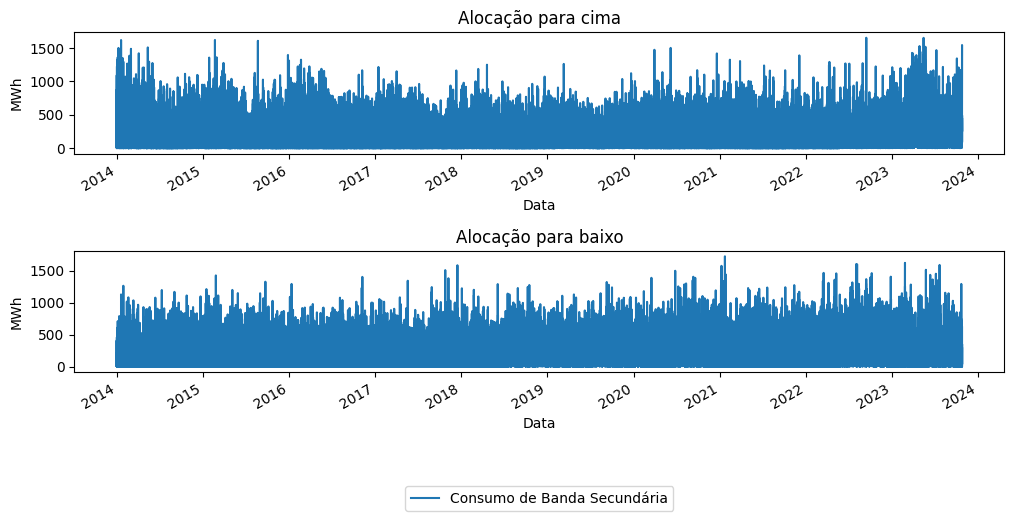
\includegraphics[width=0.6\textwidth]{plots/consumo_originais.png}
  \caption{Série Temporal dos dados alvo}
  \label{fig:targettimeseries}
\end{figure}


Para termos uma melhor percepção dos mesmos seguem, \text{infra}, quatro janelas temporais mais pequenas.

\begin{figure}[H]
  \centering
  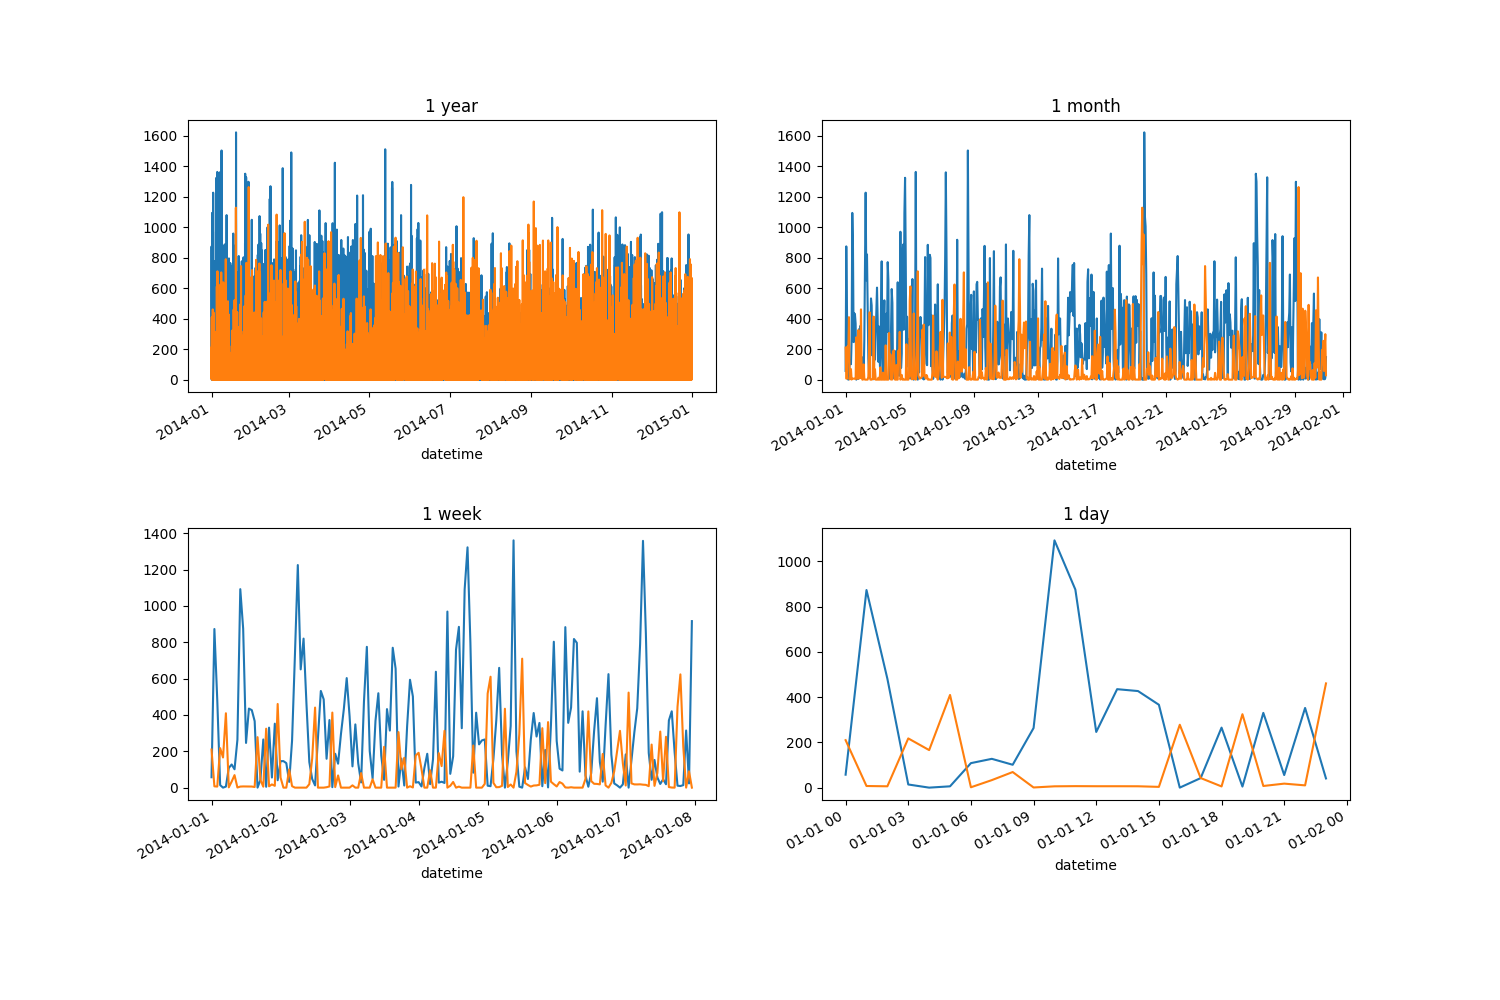
\includegraphics[width=0.7\textwidth]{plots/target_timeseries_windows.png}
  \caption{Janelas Temporais dos dados alvo}
  \label{fig:targettimeserieswindows}
\end{figure}


Da análise destas janelas temporais verificou-se claramente que ambos os atributos mantêm um comportamento tanto discreto, como linear, isto é, que ou existe algum valor, ou é zero, e se existe valor este tem comportamento linear.\par
A distribuição destes dados é claramente exponencial, o que é importante para a escolha de alguns parâmetros na modelação.\par

		
\begin{figure}[H]
  \centering
  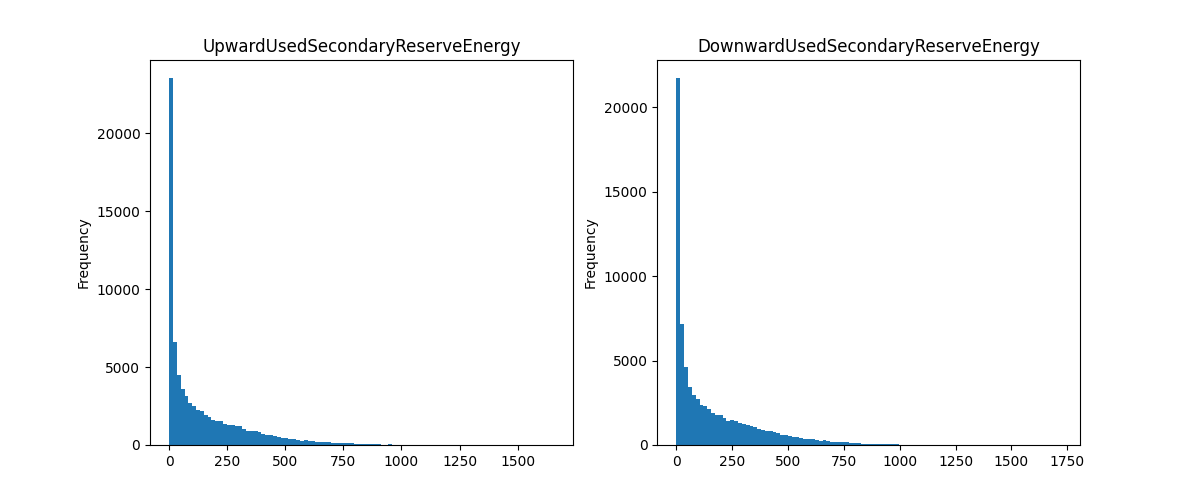
\includegraphics[width=0.6\textwidth]{plots/target_histograms.png}
  \caption{Frequência dos dados alvos}
  \label{fig:targethistograms}
\end{figure}


\paragraph{Correlações}
\text{ }  \par

Os modelos vão depender bastante de correlação entre variáveis.

Nesta secção procuramos identificar se há visiveis relações entre as variáveis, e se há relações temporais  visiveis nas colunas alvo.


\subparagraph{Correlações entre atributos}
\text{ }  \par


\begin{figure}[H]
  \centering
  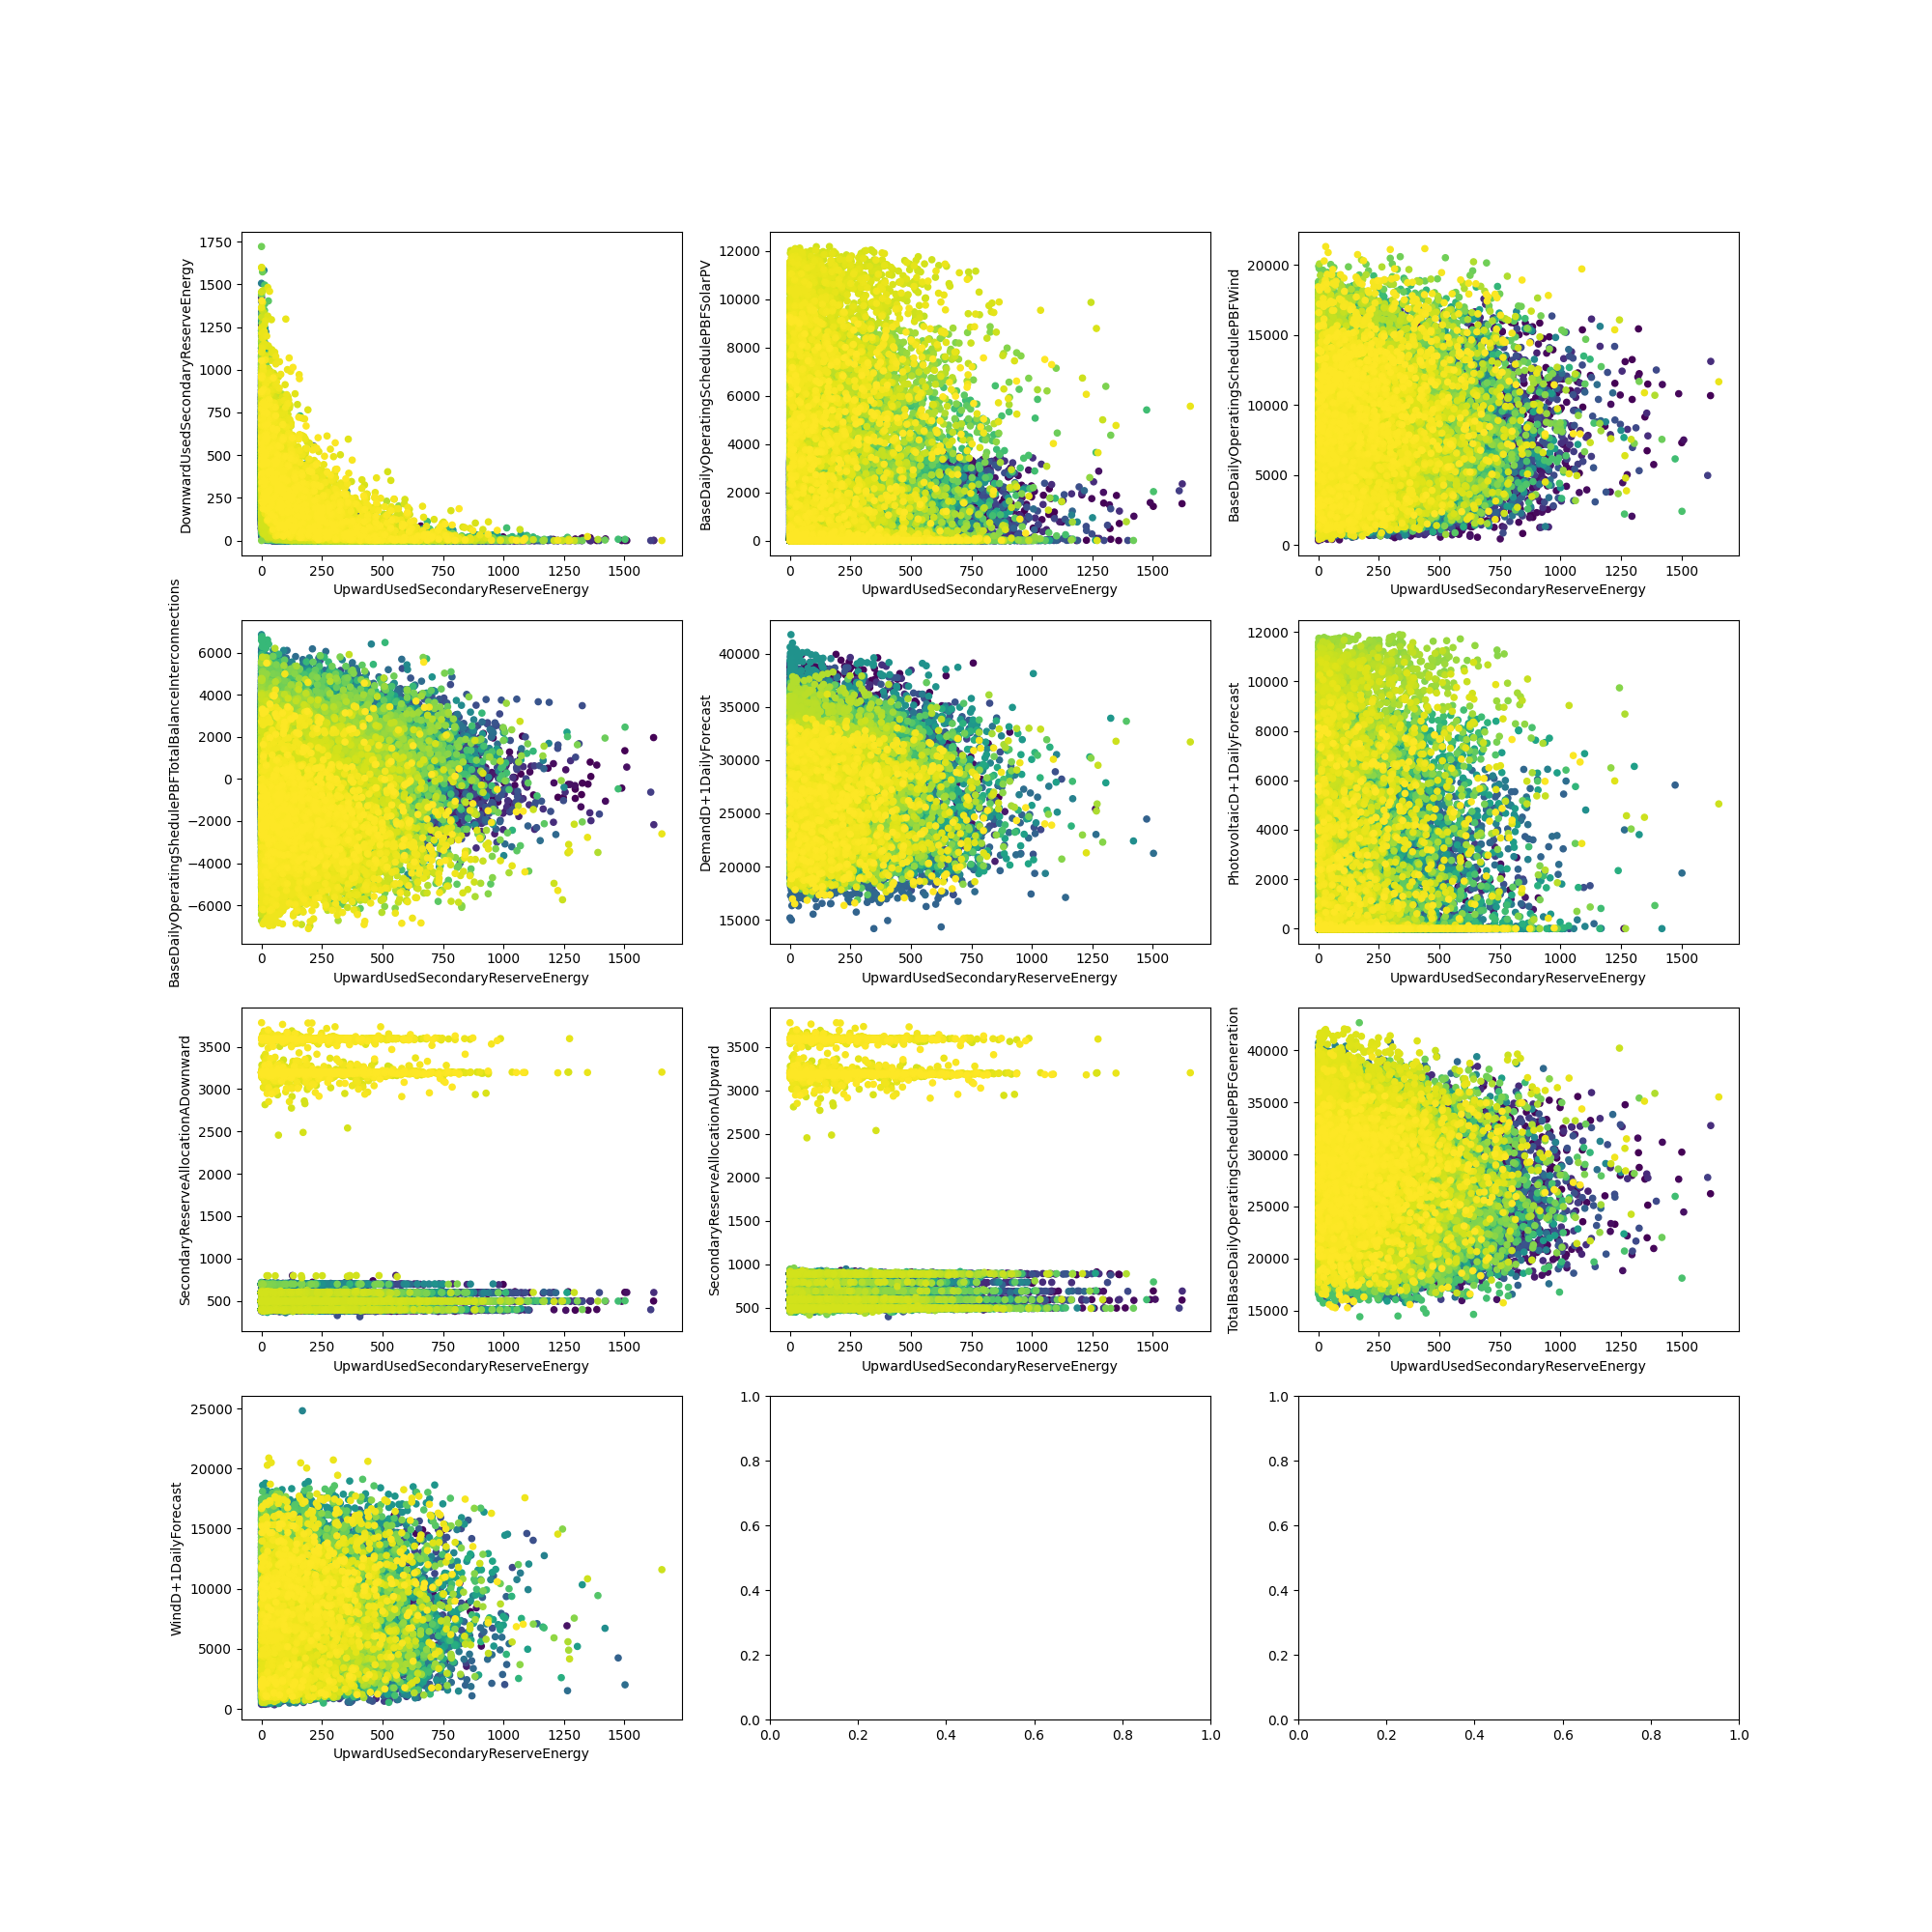
\includegraphics[width=0.90\textwidth]{plots/feature_correlation.png}
  \caption{Correlação entre atributos}
  \label{fig:featurecorrelation}
\end{figure}

Esta figura apresenta a dispersão de valores entre a energia usada, primeiras três linhas a energia para cima e as seguintes a energia para baixo, e os outros atributos presentes.\par
As correlações entre variáveis parecem muitos escassas, o que já apresenta que a previsão destes dados, usando estas variáveis, será ser um problema difícil.\par
Por norma, é feita uma seleção de atributos baseada nestas correlações, eliminando assim os atributos que ajudam menos, ou até prejudicam os modelos.\par
Seguem, \textit{infra}, os valores de correlação é possível verificar numericamente que existe muito pouca correlação entre os atributos. Onde a primeira coluna são os valores de correlação para a energia usada a subir e a segunda coluna as correlações da energia usada a descer.\par

\begin{figure}[H]
  \centering
  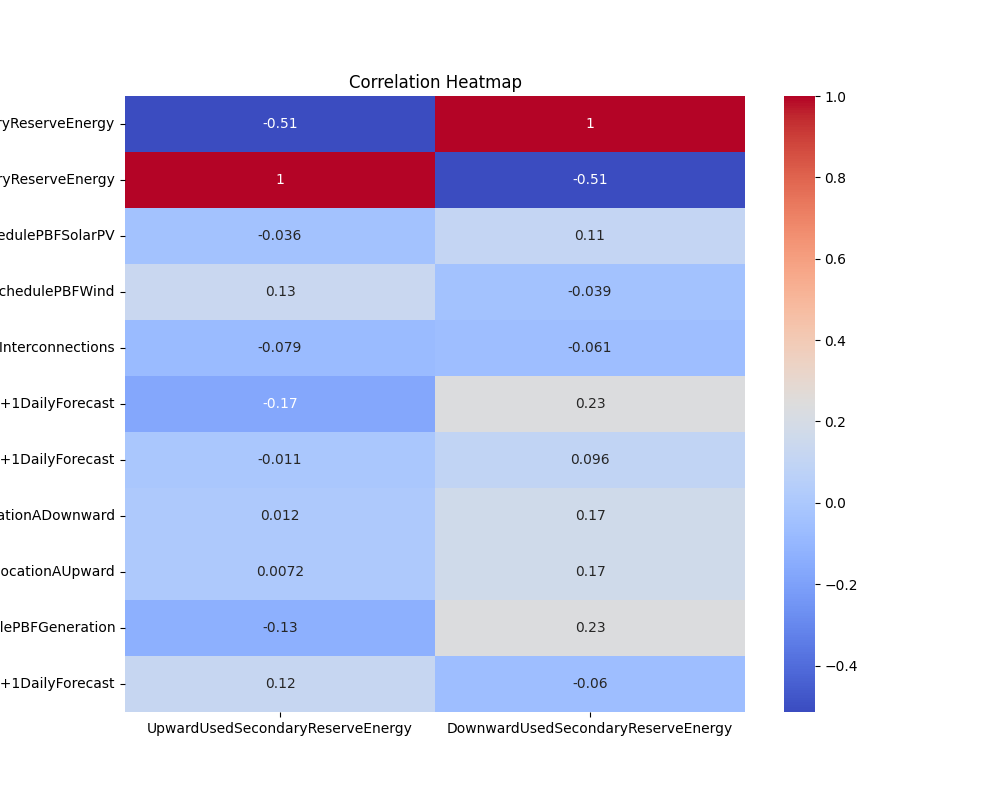
\includegraphics[width=\textwidth]{plots/correlation_heatmap.png}
  \caption{Valores de correlação entre atributos}
  \label{fig:correlationheatmap}
\end{figure}

\subparagraph{Correlações Temporais}
\text{ }  \par

\begin{figure}[H]
  \centering
  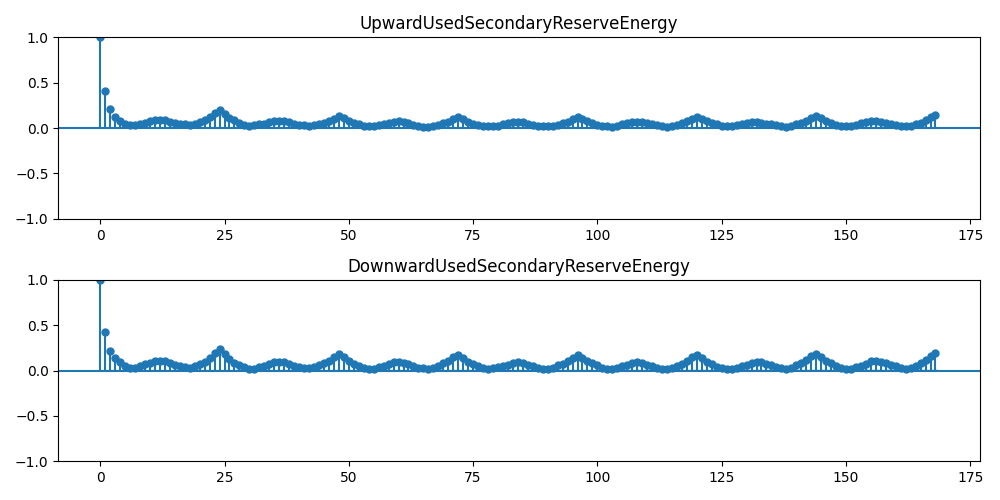
\includegraphics[width=0.75\textwidth]{plots/autocorrelation.png}
  \caption{Autocorrelação Temporal}
  \label{fig:autocorrelation}
\end{figure}

A autocorrelação, em ambos os alvos, é mais forte nas 3 horas mais próximas, e nos pontos com diferença de 12 e 24 horas.\par
É de notar que estes valores são baixos, prometendo já também uma baixa regressividade temporal.\par
Os melhores saltos temporais e suas correlações são mostradas na tabelas em baixo:\\


\begin{table}[H]
  \caption{Autocorrelação Temporal}    
  \resizebox{\linewidth}{!}{\begin{tabular}{lllllllllll}
\toprule
\midrule
\multirow[t]{2}{*}{UpwardUsedSecondaryReserveEnergy} & horas & 1 & 2 & 24 & 23 & 25 & 168 & 144 & 192 & 48 \\
 & rácio & 0.44 & 0.24 & 0.22 & 0.19 & 0.19 & 0.17 & 0.16 & 0.16 & 0.16 \\
\cline{1-11}
\multirow[t]{2}{*}{DownwardUsedSecondaryReserveEnergy} & horas & 1 & 2 & 24 & 23 & 25 & 168 & 144 & 192 & 48 \\
 & rácio & 0.43 & 0.22 & 0.25 & 0.20 & 0.19 & 0.21 & 0.19 & 0.20 & 0.19 \\
\cline{1-11}
\bottomrule
\end{tabular}
}
  \label{tab:tempcorr}
  \end{table}

Outro ponto a denotar é que os objectos não têm um comportamento completamente linear, i.e., parece existir um comportamento discreto na questão ser alocado ou não esta reservas secundárias, e caso seja alocado, aí existir alguma linearidade.\par
Logo qualquer tipo de modelação terá de resolver primeiramente este problema.\par
Da análise destas relações, é possível verificar que em termos de atributos usados será um desafio complicado para qualquer tipo de modelo.\par
No âmbito desta dissertação pretendemos verificar a qualidade das previsões usando estes mesmo atributos, pelo que, não será feita seleção dos mesmos.\par
A nível da relação temporal, a maior parte dos modelos que testaremos aplica um janela na dimensão temporal, usando todos os valores nessa janela, e aplicando os pesos nessas distâncias que mais se enquadram. Logo também não é relevante escolher apenas as distâncias temporais com maior correlação, pois os modelos farão essa pesagem.\par


 \label{se:dadoscrus}



\thispagestyle{plain}



\subsubsection{Tratamento dos dados}

\paragraph{Normalização} \par
\text{ }  \par

A normalização foi deixada para ser aprendida nos modelos, sendo que todos os modelos têm a normalização como segunda camada.\par

\paragraph{Limpeza} \par
\text{ }  \par

Podemos ver pelos gráficos seguintes que a existem alguns \textit{outliers}, sendo estes definidos como 3 (três) desvios padrão de distância à média.\par
Estes gráficos mostram também que existe uma variação do que são os valores normais de cada atributo a nível temporal. Logo um método de limpeza não se poderia basear apenas numa definição geral de \textit{outliers}, mas teria também de ser feito em janelas temporais.\par
Pelo mesmo argumento e visto que os \textit{outliers} fazem parte do que queremos também descobrir, não é aplicada nenhum método de remoção dos mesmo, sendo os dados passados a cru para os modelos.\par


\begin{figure}[H]
  \centering
  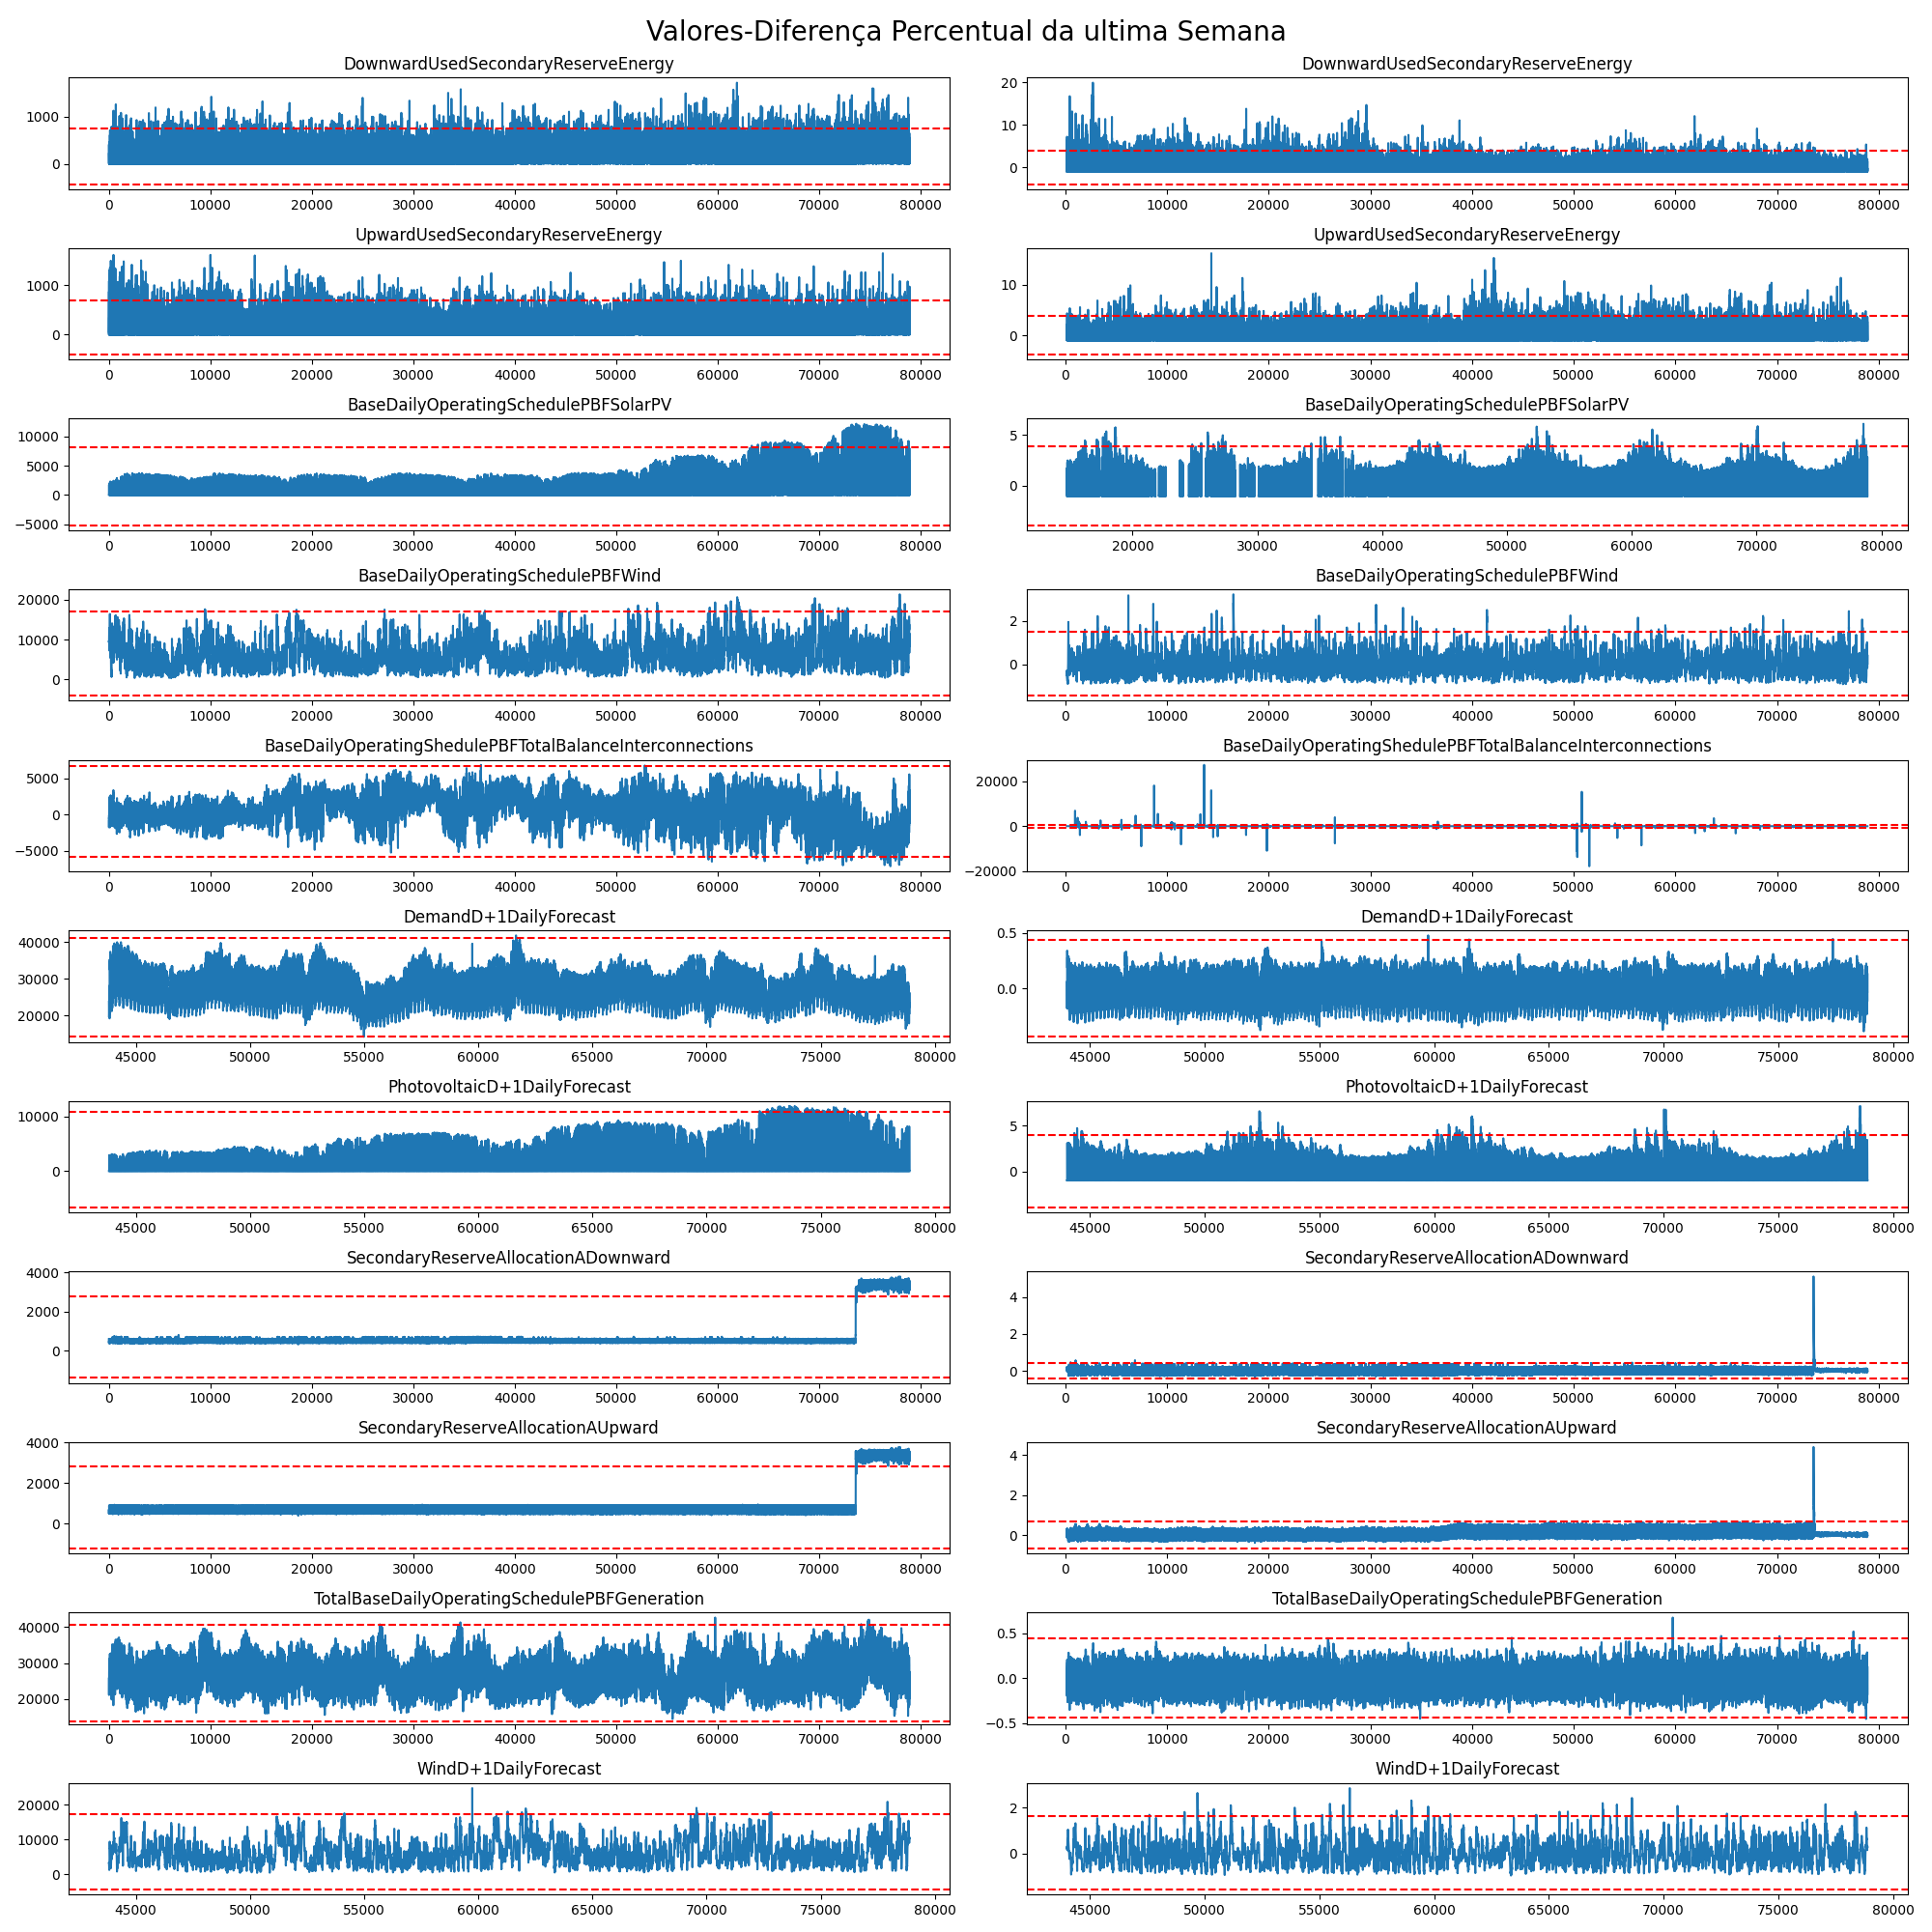
\includegraphics[width=\textwidth]{plots/Outliers_3stds.png}
  \caption{Outliers}
\end{figure}

Com outra análise desta variação dos atributos a nível temporal verificou-se que qualquer divisão dos dados para treino e teste deva levar as variações em consideração. Com efeito, o treino deve ter representatividade de todas as condições diferentes, ou pelo menos, da maior parte delas.\par


\paragraph{Dados em falta (\textit{Missing Data})}
\text{ }  \par

Estudemos também o caso de dados em falta. Alguns destes atributos têm certas entradas vazias, e como é possível verificar, alguns não têm determinados anos inteiros.\par
Como é nossa intenção usar o máximo de dados possíveis, usaremo nesses dados usar técnicas de \textit{imputing}.\par
Vendo no gráfico abaixo, verificamos que temos dados em falta de vários anos, em três atributos, e um deles tem algumas horas esporádicas em falta nos primeiros anos.\par

\begin{figure}[H]
  \centering
  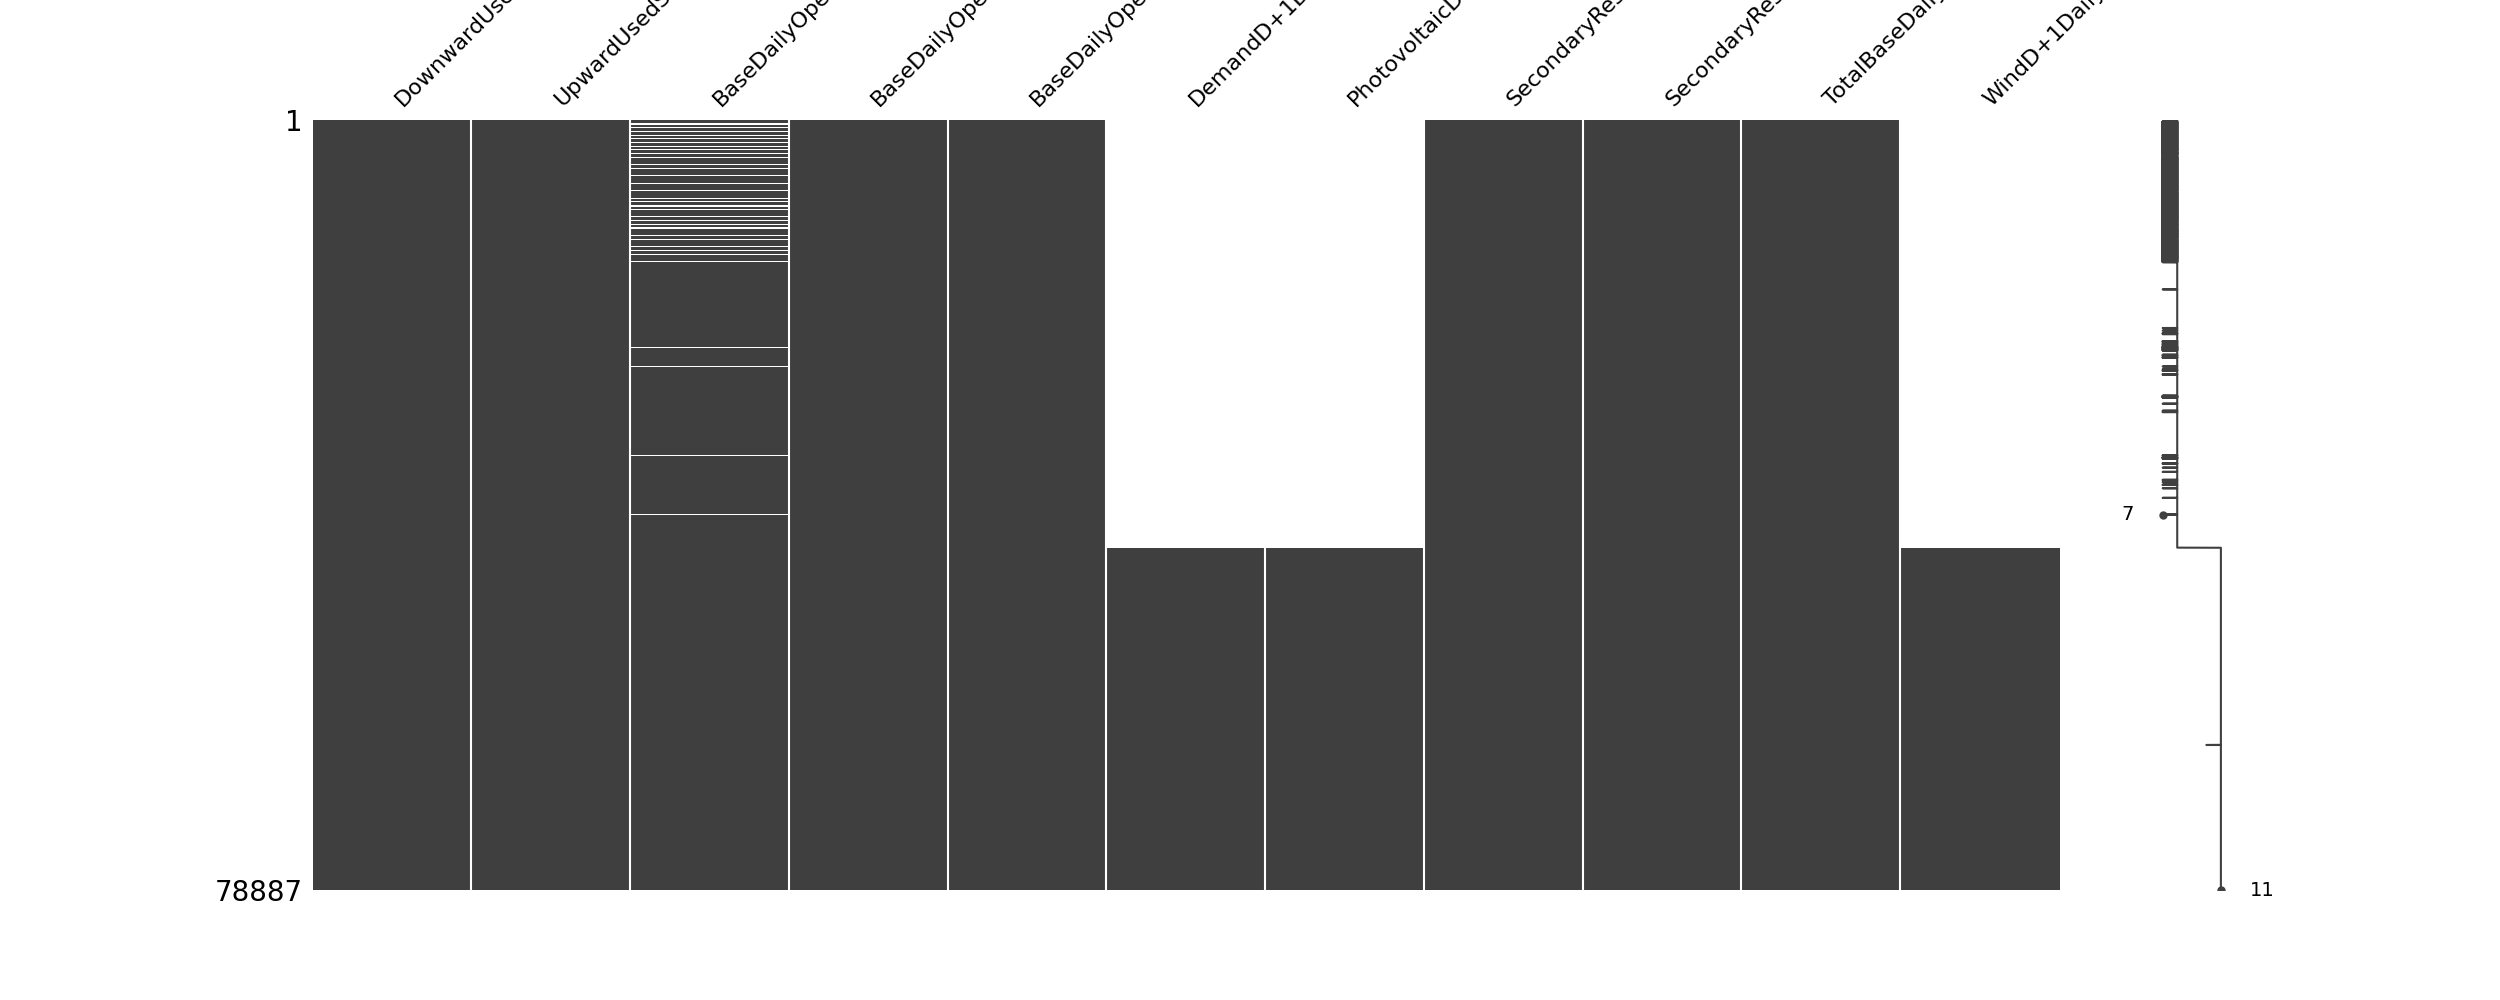
\includegraphics[width=\textwidth]{plots/missing_data.png}
  \caption{Dados em falta}
\end{figure}

Vamos aplicar o método experimental \href{https://scikit-learn.org/stable/modules/generated/sklearn.impute.IterativeImputer.html}{IterativeImputer} da biblioteca de \textit{python} \href{https://scikit-learn.org/stable/index.html}{sklearn}.\par
Este método é baseado nos trabalhos de \cite{vanBuuren2011} e de \cite{Buck1960}.\par
Por ultimo foi adicionado ao dados mais atributos, sendo eles todos de cariz temporal. São adicionados atributos correspondentes à hora, ao dia do ano, ao dia da semana, ao dia do mês, mês, ano.\par

 \label{se:tratamentodados}

\subsubsection{Dados de treino}

Após o tratamento apresentado as estatísticas gerais dos dados usados para treinar o modelo são:

\begin{table}[H]
    \centering
    \caption{Dados de Treino}    
    \resizebox{\linewidth}{!}{\begin{table}[H] 
    \caption{Training data summary. \label{training_data_sum}}
    \newcolumntype{C}{>{\centering\arraybackslash}X}
    \begin{tabularx}{\textwidth}{CCCCC}
    \toprule
    & \textbf{mean}	& \textbf{std}	& \textbf{min} & \textbf{max}\\
    \midrule
    Down Used & 168.20 & 199.67 & 0.00 & 1721.40 \\
    Up Allocated & 662.94 & 150.62 & 399.00 & 958.00 \\
    Down Allocated & 549.27 & 126.67 & 312.00 & 956.00 \\
    Up Used & 158.10 & 191.62 & 0.00 & 1654.80 \\
    DA Wind & 5824.12 & 3413.15 & 71.33 & 20879.30 \\
    DA PV & 1666.31 & 2719.60 & 0.00 & 14925.30 \\
    DA Demand & 27944.24 & 4479.39 & 14170.00 & 41773.00 \\
    DA Schedule Generation & 27249.43 & 4603.58 & 13470.50 & 42707.60 \\
    DA Schedule PV Generation & 1714.09 & 2815.35 & 0.00 & 16358.90 \\
    DA Schedule Wind Generation & 6525.51 & 3582.36 & 308.60 & 21619.60 \\
    DA Scheduled Tie Lines & 290.58 & 2157.11 & -7817.00 & 6858.50 \\
    \bottomrule
    \end{tabularx}
    % \noindent{\footnotesize{\textsuperscript{1} Tables may have a footer.}}
\end{table}

}
    \end{table}


\thispagestyle{plain}
\subsection{Dados de Validação}
Os dados de validação são os meses após os dados de treino, de Janeiro 2024 ao fim de Agosto 2024.\par
Usamos como \textit{benchmark} as capacidades alocadas, "\textit{SecondaryReserveAllocationAUpward}" e "\textit{SecondaryReserveAllocationADownward}", e como validação e objectivo, \hyperref[se:metneuralnet]{y}, a própria energia usada, "\textit{UpwardUsedSecondaryReserveEnergy}" e "\textit{DownwardUsedSecondaryReserveEnergy}".

\begin{figure}[H]
    \centering
    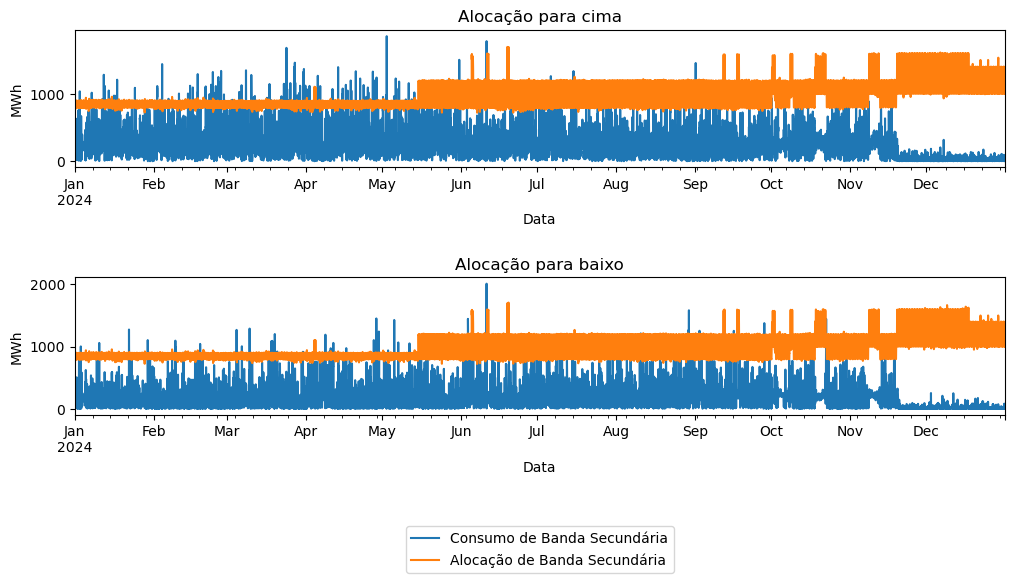
\includegraphics[width=0.6\textwidth]{plots/benchmark_alocacoes_validacao.png}
    \caption{Série Temporal dos dados de Benchmark c/ consumo real}
    \label{fig:benchmarktimeseries}
\end{figure}

Os valores alocados no período de validação mantêm um dinamismo fixo entre dois pontos, seguindo um formula não dinamica. \par
Mas o mais importante a notar é a forma estática destes métodos, que, em virtude da natureza flutuante da energia necessária, apresentam, frequentemente um erro grande.\par
Tal é possível de verificar através da análise de algumas janelas temporais dentro do período de validação, em concreto, atentando no melhor e pior resultado, em termos de erro absoluto, em janelas temporais de ano, mês, semana e dia.\par


\begin{figure}[H]
    \centering
    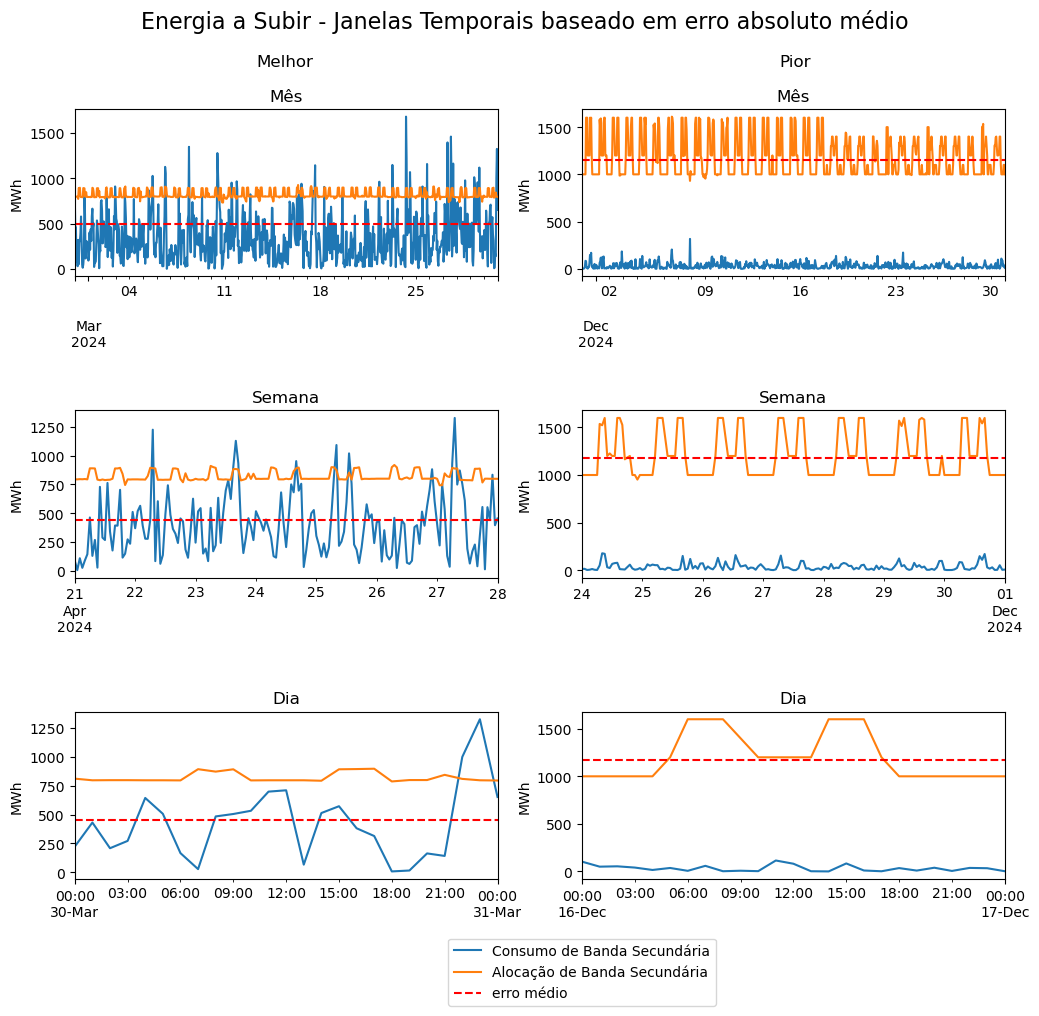
\includegraphics[width=0.7\textwidth]{plots/alocacoes_temporais_upward_dataset.png}
    \caption{Janelas temporais de \textit{benchmark} energia a subir}
    \label{fig:benchmarktimewindowsup}
\end{figure}


\begin{figure}[H]
    \centering
    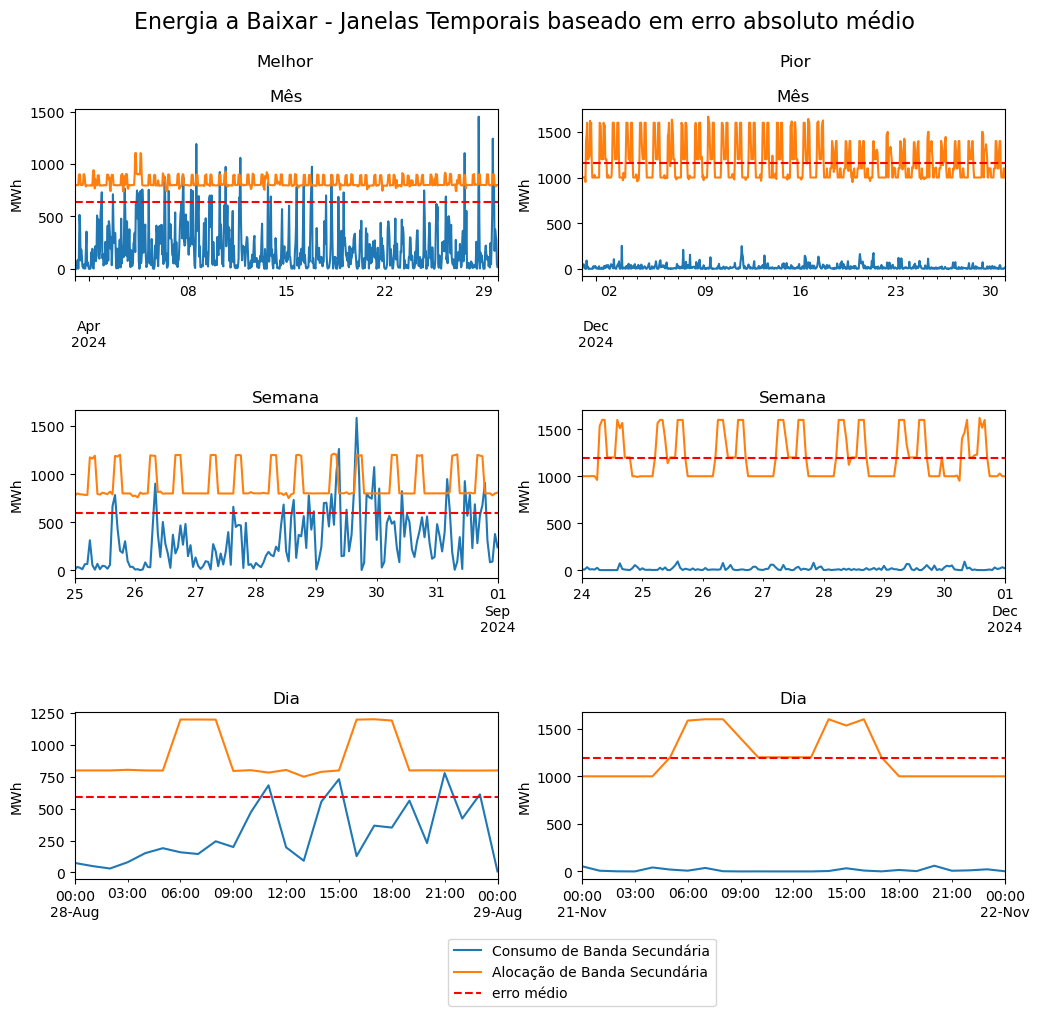
\includegraphics[width=0.7\textwidth]{plots/alocacoes_temporais_downward_dataset.png}
    \caption{Janelas temporais de \textit{benchmark} energia a descer}
    \label{fig:benchmarktimewindowsdown}
\end{figure}

Dentro destas janelas temporais conseguimos ter melhor a percepção da natureza estática deste modelo actual, e quão longe está dos valores reais necessários.\par

Os resultados a melhorar são:\\
\begin{table}[H]
    \centering
    \caption{Resultados métricas \textit{benchmark}}    
    \resizebox{0.8\linewidth}{!}{\begin{table}[H] 
    \caption{This is a table caption. Tables should be placed in the main text near to the first time they are~cited.\label{tab1}}
    \newcolumntype{C}{>{\centering\arraybackslash}X}
    \begin{tabularx}{\textwidth}{CCCCC}
    \toprule
    & \textbf{RMSE}	& \textbf{SAE}	& \textbf{AllocF} & \textbf{AllocD}\\
    \midrule
    Up Allocation (MW) & 536.55 & 17357826.75 & 152679.00 & 17205147.75 \\
    Down Allocation (MW) & 408.99 & 12981575.55 & 479191.60 & 12502383.95 \\
        \bottomrule
    \end{tabularx}
    % \noindent{\footnotesize{\textsuperscript{1} Tables may have a footer.}}
\end{table}

}
    \label{tab:benchmarkmetrics}
    \end{table}

As correlações entre o método actual e a energia consumida podem ser vistas na figura abaixo:\\


\begin{figure}[H]
    \centering
    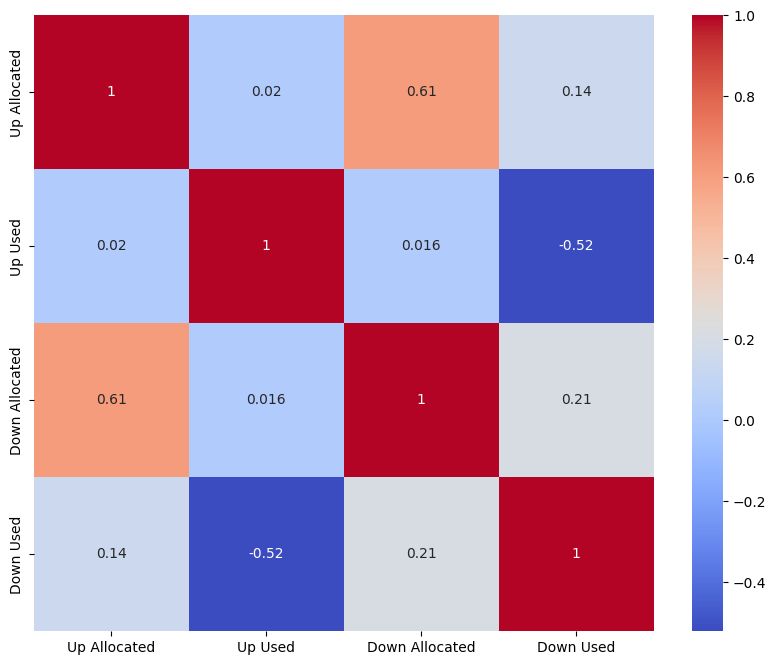
\includegraphics[width=\textwidth]{plots/correlation_heatmap_benchmark.png}
    \caption{Correlação entre \textit{benchmark} e real}
    \label{fig:benchmarkcorr}
\end{figure}

% TODO: meter formula da previsão ENTO-e no capitulo estudo 2 -> nao existe publicamente
Neste período de validação, a energia alocado para cima é igual a alocada para baixo. com uma correlação de 1, diferente da totalidade dos dados disponíveis em que as alocações mostram uma correlação de 58\%.
As relações entre as energias alocadas são altas devido à natureza do \hyperref[]{método de previsão} enquanto que a correlação entre a energia alocada e a usada são bastante baixas com 23\% na alocaçao a descer e 9,8\% na alocação a subir.\par
O que não mostra uma ligaçao entre as alocações e a energia usada, mas apenas entre as energias alocadas.\par

 \label{se:val_data}
